\documentclass[a4paper,10pt,twocolumn]{article}

\usepackage[utf8x]{inputenc}
\usepackage[french]{babel}
\usepackage{graphicx,times}
\usepackage[T1]{fontenc}
\usepackage{amsmath}
\usepackage[font=footnotesize]{caption}
\usepackage{fancyhdr}
\usepackage[explicit]{titlesec}
\usepackage{hyperref}
%\usepackage[square,comma,numbers]{natbib}
\usepackage{tabularx}

\newcolumntype{L}[1]{>{\raggedright\arraybackslash}p{#1}}
\newcolumntype{C}[1]{>{\centering\arraybackslash}p{#1}}
\newcolumntype{R}[1]{>{\raggedleft\arraybackslash}p{#1}}

%\renewcommand{\bibsection}{}
%\def\bibfont{\footnotesize}
%\setlength{\bibsep}{0.2em}
%\setlength{\bibhang}{10em}

\hypersetup{colorlinks=true, urlcolor=blue, urlbordercolor={0 0 1}, citecolor=black, citebordercolor={1 1 1}}

\addto\captionsfrench{\def\figurename{Fig.}}
\addto\captionsfrench{\def\tablename{Tableau}}

\captionsetup[figure]{labelsep=period, justification=raggedright, singlelinecheck=false}
\captionsetup[table]{labelsep=period, justification=centering, singlelinecheck=false}

\parindent 10pt

\setlength{\voffset}{-1.3in}
\setlength{\topmargin}{1.25cm}
\setlength{\headheight}{1.125cm}
\setlength{\headsep}{0cm}

\setlength{\hoffset}{-1in}
\setlength{\oddsidemargin}{1.3cm}
\setlength{\evensidemargin}{1.3cm}

\setlength{\textheight}{25cm}%23.5
\setlength{\textwidth}{18.5cm}

\setlength{\headsep}{0.67cm}
\setlength{\columnwidth}{8.75cm}
\setlength{\columnsep}{0.63cm}

\setlength{\abovecaptionskip}{0em}
\setlength{\belowcaptionskip}{0em}

\titleformat{\section}
  {\normalfont}{\thesection.}{0.5em}{\MakeUppercase{#1}}
\titleformat{\subsection}
  {\normalfont\itshape}{\thesubsection.}{1.5em}{#1}
\titleformat{\subsubsection}
  {\normalfont\itshape}{\thesubsubsection.}{1.5em}{#1}
	
\titlespacing\section{0pt}{1em}{0.5em}
\titlespacing\subsection{0pt}{1em}{0.5em}
\titlespacing\subsubsection{0pt}{1em}{0.5em}

\fancyhf{}
\fancyhead[R]{\fontsize{8pt}{8pt}\selectfont \textbf{S}YMPOSIUM DE \textbf{G}ENIE \textbf{E}LECTRIQUE (SGE 2018), 3-5 JUILLET 2018, NANCY, FRANCE}
\renewcommand{\headrulewidth}{0pt}


\pagestyle{empty}


\title{
\fontsize{24pt}{24pt}\selectfont
Gestion d'énergie avec entrées incertaines : \\
quel algorithme choisir ?\\
Illustration pour un système PV-stockage.
}

\newcommand\tsp[1]{\textsuperscript{#1}}

\author{
\fontsize{11pt}{11pt}\selectfont
Pierre HAESSIG\tsp{*}\\
\fontsize{10pt}{10pt}\selectfont
\tsp{*}CentraleSupélec -- IETR
}

\date{}


\begin{document}

\maketitle
\thispagestyle{fancy}


\fontsize{9pt}{9pt}\selectfont
\textbf{RÉSUME --
Le pilotage optimal des systèmes énergétiques nécessite l'emploi d'algorithmes
de gestion optimale.
Ces outils se rattachent à théories de disciplines variées (Automatique, Optimisation, Recheche Opérationnelle),
qui ont chacune leur spécificité tout en se recouvrant partiellement.
%
Il est donc difficile, pour la personne ``non initiée'', de saisir les principales caractéristiques
de chaque approche pour pouvoir les comparer et finalement trouver
quelles méthodes sont plus adaptées à un problème donné.
%
Nous proposons ici, sur un exemple simple de système photovoltaïque-stockage, de
comparer différentes méthodes en soulignant en particulier les investissements
en temps à prévoir :
temps pour la compréhension du cadre théorique,
temps pour la modélisation du problème dans ce cadre,
temps pour l'implémentation numérique et la validation des résultats.
Nous soulignons également quelques pièges typiques, comme l'optimisation
déterministe anticipative dans un contexte stochastique.
}\\

\textbf{\textit{Gestion d'énergie, Optimisation dynamique, Optimisation stochastique,
Commande prédictive, Programmation Dynamique}}

\fontsize{10pt}{10pt}\selectfont


\section{Introduction}

Décrire le contexte et les objectifs du travail. Positionner le travail par rapport à la littérature et aux principaux travaux antérieurs. Présenter le plan de la communication. (Style ‘Normal’).
\cite{Haessig:2014:PhD}


\section{Approches d'optimisation}

Développer dans les sections, sous-sections et sous sous-sections (ne pas excéder 3 niveaux hiérarchiques) les travaux réalisés en présentant les grandes étapes et les principaux résultats.

\textbf{Le résumé final de la communication doit comporter au maximum 2 pages et doit respecter le format décrit dans ce document. La taille du fichier pdf est par ailleurs limitée à 3.5 Mo.}


TODO: cite

* sareni sge 2014
* thèse geeps voiture

\subsection{Programmation dynamique}
bon cadre théorique,
pb à l'implémentation

\subsection{Optimisation déterministe anticipative}
le piège

\subsection{MPC déterministe}
le classique

\subsection{MPC stochastique et robuste}


\subsection{Commande prédictive non-linéaire}

Optimica JModelica.org \cite{Akesson:2010:CCE}

\begin{figure}[!ht]
	\begin{center}
		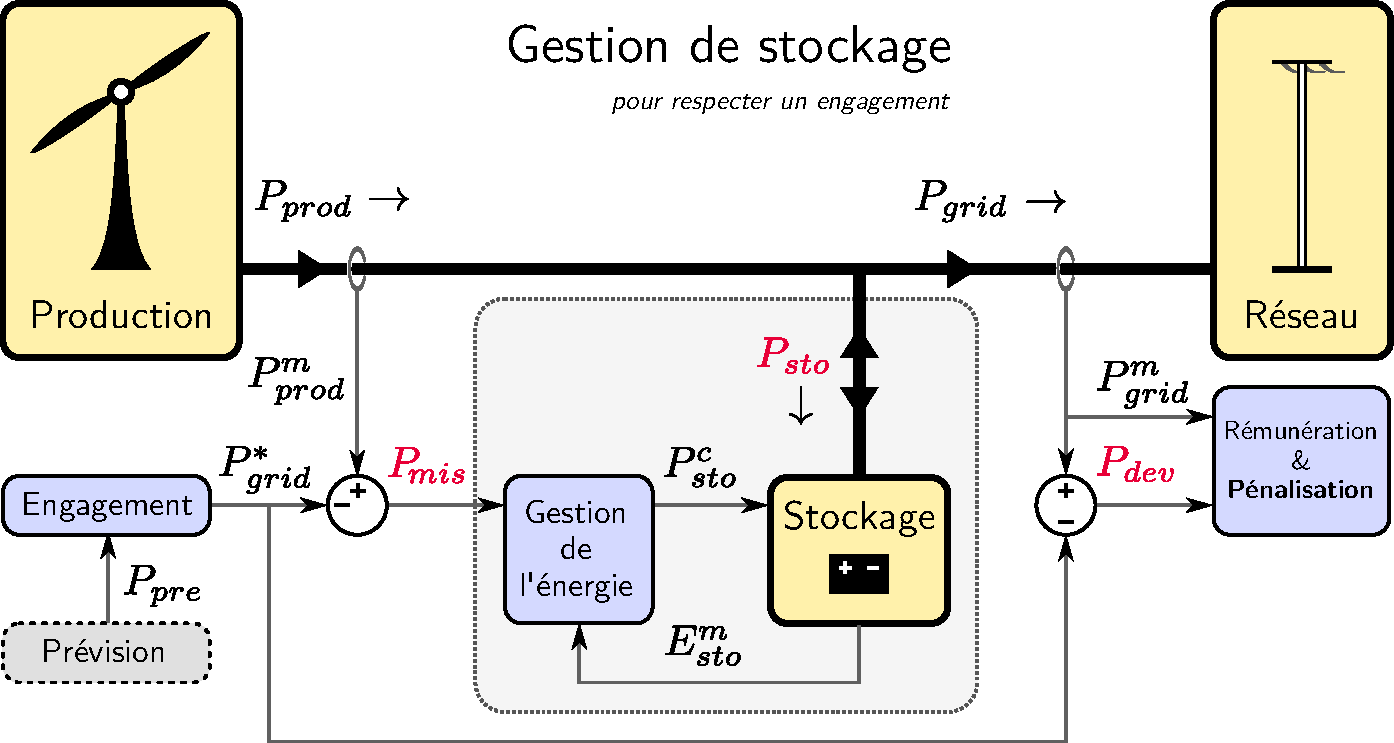
\includegraphics[width=0.6\columnwidth]{figures/wind_storage.pdf}
	\end{center}
	
	\caption{Titre de la figure (Style ‘Légende’)}
	\label{fig_1}
\end{figure}

\begin{table}[!h]
	\caption{Mettre ici le titre du tableau}
	
	\begin{center}
		\begin{tabular}{|>{\footnotesize}L{1.4cm}|>{\footnotesize}L{1.5cm}|>{\footnotesize}L{2.4cm}|>{\footnotesize}L{2.1cm}|}
			\hline
			\textbf{Titre colonne 1} & \textbf{Titre colonne 2} & \textbf{Style (‘Titre colonnes tableaux’)} & \textbf{} \\
			\hline
			Donnée 1 & Style (Cellules tableaux’) & & \\
			\hline
			Donnée 2 & & & \\
			\hline
		\end{tabular}
	\end{center}
	
	\label{tab_1}
\end{table}


\begin{equation}
	y = f(x) + \sum_{k=1}^{\infty} h_k \cdot sin(k \omega t)
	\label{eq_1}
\end{equation}


\section{Soumission de la communication}

La soumission se fait en ligne à partir du site électronique de la conférence : \url{http://sge2018.sciencesconf.org} (voir la rubrique ‘Soumission en ligne des communications’).\\

Le fichier soumis sera préalablement converti au format PDF avec les polices incorporées et ne devra pas excéder la taille maximale de 3.5 Mo.


\section{Conclusions}

Rappeler les principaux résultats marquants et originaux du travail. Le cas échéant, proposer des perspectives au travail présenté.


\section{Remerciements}

Cette partie (facultative) doit être placée entre la conclusion et les références.


\bibliographystyle{IEEEtran}
\bibliography{00_References}


\end{document}

